\documentclass[dvipdfmx]{jsarticle}
\setcounter{section}{3}
\setcounter{subsection}{1}
\usepackage{xr}
\externaldocument{8.1.3}
\externaldocument{8.1.6}
\externaldocument{8.3.1}
\usepackage{amsmath,amsfonts,amssymb,array,comment,mathtools,url,docmute}
\usepackage{longtable,booktabs,dcolumn,tabularx,mathtools,multirow,colortbl,xcolor}
\usepackage[dvipdfmx]{graphics}
\usepackage{bmpsize}
\usepackage{amsthm}
\usepackage{enumitem}
\setlistdepth{20}
\renewlist{itemize}{itemize}{20}
\setlist[itemize]{label=•}
\renewlist{enumerate}{enumerate}{20}
\setlist[enumerate]{label=\arabic*.}
\setcounter{MaxMatrixCols}{20}
\setcounter{tocdepth}{3}
\newcommand{\rotin}{\text{\rotatebox[origin=c]{90}{$\in $}}}
\newcommand{\amap}[6]{\text{\raisebox{-0.7cm}{\begin{tikzpicture} 
  \node (a) at (0, 1) {$\textstyle{#2}$};
  \node (b) at (#6, 1) {$\textstyle{#3}$};
  \node (c) at (0, 0) {$\textstyle{#4}$};
  \node (d) at (#6, 0) {$\textstyle{#5}$};
  \node (x) at (0, 0.5) {$\rotin $};
  \node (x) at (#6, 0.5) {$\rotin $};
  \draw[->] (a) to node[xshift=0pt, yshift=7pt] {$\textstyle{\scriptstyle{#1}}$} (b);
  \draw[|->] (c) to node[xshift=0pt, yshift=7pt] {$\textstyle{\scriptstyle{#1}}$} (d);
\end{tikzpicture}}}}
\newcommand{\twomaps}[9]{\text{\raisebox{-0.7cm}{\begin{tikzpicture} 
  \node (a) at (0, 1) {$\textstyle{#3}$};
  \node (b) at (#9, 1) {$\textstyle{#4}$};
  \node (c) at (#9+#9, 1) {$\textstyle{#5}$};
  \node (d) at (0, 0) {$\textstyle{#6}$};
  \node (e) at (#9, 0) {$\textstyle{#7}$};
  \node (f) at (#9+#9, 0) {$\textstyle{#8}$};
  \node (x) at (0, 0.5) {$\rotin $};
  \node (x) at (#9, 0.5) {$\rotin $};
  \node (x) at (#9+#9, 0.5) {$\rotin $};
  \draw[->] (a) to node[xshift=0pt, yshift=7pt] {$\textstyle{\scriptstyle{#1}}$} (b);
  \draw[|->] (d) to node[xshift=0pt, yshift=7pt] {$\textstyle{\scriptstyle{#2}}$} (e);
  \draw[->] (b) to node[xshift=0pt, yshift=7pt] {$\textstyle{\scriptstyle{#1}}$} (c);
  \draw[|->] (e) to node[xshift=0pt, yshift=7pt] {$\textstyle{\scriptstyle{#2}}$} (f);
\end{tikzpicture}}}}
\renewcommand{\thesection}{第\arabic{section}部}
\renewcommand{\thesubsection}{\arabic{section}.\arabic{subsection}}
\renewcommand{\thesubsubsection}{\arabic{section}.\arabic{subsection}.\arabic{subsubsection}}
\everymath{\displaystyle}
\allowdisplaybreaks[4]
\usepackage{vtable}
\theoremstyle{definition}
\newtheorem{thm}{定理}[subsection]
\newtheorem*{thm*}{定理}
\newtheorem{dfn}{定義}[subsection]
\newtheorem*{dfn*}{定義}
\newtheorem{axs}[dfn]{公理}
\newtheorem*{axs*}{公理}
\renewcommand{\headfont}{\bfseries}
\makeatletter
  \renewcommand{\section}{%
    \@startsection{section}{1}{\z@}%
    {\Cvs}{\Cvs}%
    {\normalfont\huge\headfont\raggedright}}
\makeatother
\makeatletter
  \renewcommand{\subsection}{%
    \@startsection{subsection}{2}{\z@}%
    {0.5\Cvs}{0.5\Cvs}%
    {\normalfont\LARGE\headfont\raggedright}}
\makeatother
\makeatletter
  \renewcommand{\subsubsection}{%
    \@startsection{subsubsection}{3}{\z@}%
    {0.4\Cvs}{0.4\Cvs}%
    {\normalfont\Large\headfont\raggedright}}
\makeatother
\makeatletter
\renewenvironment{proof}[1][\proofname]{\par
  \pushQED{\qed}%
  \normalfont \topsep6\p@\@plus6\p@\relax
  \trivlist
  \item\relax
  {
  #1\@addpunct{.}}\hspace\labelsep\ignorespaces
}{%
  \popQED\endtrivlist\@endpefalse
}
\makeatother
\renewcommand{\proofname}{\textbf{証明}}
\usepackage{tikz,graphics}
\usepackage[dvipdfmx]{hyperref}
\usepackage{pxjahyper}
\hypersetup{
 setpagesize=false,
 bookmarks=true,
 bookmarksdepth=tocdepth,
 bookmarksnumbered=true,
 colorlinks=false,
 pdftitle={},
 pdfsubject={},
 pdfauthor={},
 pdfkeywords={}}
\begin{document}
%\hypertarget{ux53efux5faeux5206ux5199ux50cf}{%
\subsection{$C^{s}$級写像}%\label{ux53efux5faeux5206ux5199ux50cf}}
%\hypertarget{csux7d1aux95a2ux6570}{%
\subsubsection{$C^{s}$級写像}%\label{csux7d1aux95a2ux6570}}
\begin{dfn}\label{写像はCs級であることの定義}
$n$次元$C^{r}$級多様体$\left( \mathcal{M},\mathfrak{O} \right)$、$U \in \mathfrak{O}$なるその多様体$\left( \mathcal{M},\mathfrak{O} \right)$から1次元Euclid空間$E$における位相空間$\left( \mathbb{R},\mathfrak{O}_{d_{E}} \right)$への連続写像$f:U \rightarrow \mathbb{R}$、その多様体$\left( \mathcal{M},\mathfrak{O} \right)$の$C^{r}$級座標近傍系$\left\{ \left( U_{\alpha},\psi_{\alpha} \right) \right\}_{\alpha \in A}$が与えられたとき、$\forall p\in U\exists\alpha \in A$に対し、$p \in U_{\alpha}$が成り立つのであった。さらに、$\exists V \in \mathbf{V} \left(p\right) $に対し、$V \subseteq U \cap U_{\alpha}$も成り立つのであった。このとき、関数$f \circ \psi_{\alpha}^{- 1}|V\left( \psi_{\alpha}|V \right):V\left( \psi_{\alpha}|V \right) \rightarrow \mathbb{R}$が$s \leq r$として$C^{s}$級であるとき、その写像$f$はその元$p$で$C^{s}$級であるといいこのような写像全体の集合を$C^s_p \left( V\right) $と書く。さらに、$\forall p \in U$に対し、その写像$f$がその元$p$で$C^{s}$級であるとき、その写像$f$をその開集合$U$で$C^s$級であるといいこのような写像全体の集合を$C^s \left( U\right)$と書く\footnote{定理\ref{8.3.2.3}より実は座標近傍系の取り方に依らずに定義できることも注目すべき点になっています。}。
\end{dfn}\par
このことは次のように表される。
\begin{center}
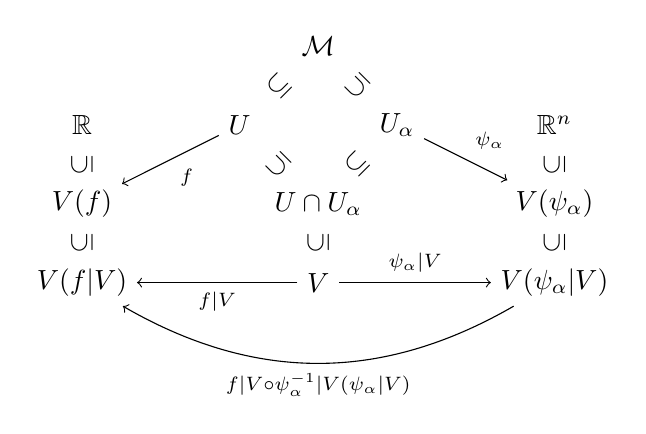
\begin{tikzpicture}[auto]
  \node (a) at ( 0, 3) {$\mathcal{M} $};
  \node (b) at (-1, 2) {$U $};
  \node (c) at ( 1, 2) {$U_\alpha $};
  \node (d) at ( 0, 1) {$U \cap U_\alpha $};
  \node (e) at ( 0, 0) {$V $};
  \node (f) at (-3, 2) {$\mathbb{R} $};
  \node (g) at (-3, 1) {$V(f) $};
  \node (h) at (-3, 0) {$V(f|V) $};
  \node (i) at ( 3, 2) {$\mathbb{R}^n $};
  \node (j) at ( 3, 1) {$V(\psi_\alpha ) $};
  \node (k) at ( 3, 0) {$V(\psi_\alpha |V ) $};
  \node (x) at (-0.5, 2.5) {\rotatebox{45}{$\subseteq $}};
  \node (x) at ( 0.5, 2.5) {\rotatebox{135}{$\subseteq $}};
  \node (x) at (-3.0, 1.5) {\rotatebox{90}{$\subseteq $}};
  \node (x) at (-0.5, 1.5) {\rotatebox{135}{$\subseteq $}};
  \node (x) at ( 0.5, 1.5) {\rotatebox{45}{$\subseteq $}};
  \node (x) at ( 3.0, 1.5) {\rotatebox{90}{$\subseteq $}};
  \node (x) at (-3.0, 0.5) {\rotatebox{90}{$\subseteq $}};
  \node (x) at ( 0.0, 0.5) {\rotatebox{90}{$\subseteq $}};
  \node (x) at ( 3.0, 0.5) {\rotatebox{90}{$\subseteq $}};
  \draw [->] (b) to node {$\scriptstyle f$} (g);
  \draw [->] (c) to node {$\scriptstyle \psi_\alpha $} (j);
  \draw [->] (e) to node {$\scriptstyle f|V$} (h);
  \draw [->] (e) to node {$\scriptstyle \psi_\alpha |V$} (k);
  \draw [->] (k) to[bend left=30] node {$\scriptstyle f|V \circ \psi_\alpha^{-1}|V(\psi_\alpha |V) $} (h);
\end{tikzpicture}
\end{center}
\begin{thm}\label{8.3.2.1}
$n$次元$C^{r}$級多様体$\left( \mathcal{M},\mathfrak{O} \right)$、その多様体$\left( \mathcal{M},\mathfrak{O} \right)$の$C^{r}$級座標近傍系$\left\{ \left( U_{\alpha},\psi_{\alpha} \right) \right\}_{\alpha \in A}$が与えられたとき、$\forall \alpha \in A$に対し、その局所座標系$\psi_\alpha $が$\psi_\alpha =\left( \psi_\alpha^i \right)_{i\in \varLambda_n }$とおかれれば、$\forall i\in \varLambda_n $に対し、その写像$\psi_\alpha^i $はその開集合$U_\alpha $で$C^r$級である。
\end{thm}
\begin{proof}
$n$次元$C^{r}$級多様体$\left( \mathcal{M},\mathfrak{O} \right)$、その多様体$\left( \mathcal{M},\mathfrak{O} \right)$の$C^{r}$級座標近傍系$\left\{ \left( U_{\alpha},\psi_{\alpha} \right) \right\}_{\alpha \in A}$が与えられたとき、$\forall \alpha \in A$に対し、その局所座標系$\psi_\alpha $が$\psi_\alpha =\left( \psi_\alpha^i \right)_{i\in \varLambda_n }$とおかれれば、$\forall i\in \varLambda_n \forall p\in U_\alpha $に対し、定理\ref{8.3.1.3}より$\exists \beta \in A$に対し\footnote{例えば、$\beta =\alpha $が挙げられる。}、$p\in U_{\alpha} \cap U_{\beta} $で、$\exists V \in \mathfrak{O}$に対し、$p\in V \subseteq U_{\alpha} \cap U_{\beta}$となるので、関数$\psi_\alpha^i \circ \psi_{\beta}^{- 1}|V\left( \psi_{\beta}|V \right):V\left( \psi_{\beta}|V \right) \rightarrow \mathbb{R}$について、$C^{r}$級多様体の定義より座標変換$f_{\left( U_{\beta},\psi_{\beta} \right) \rightarrow \left( U_{\alpha},\psi_{\alpha} \right)}$がその定義域で$C^{r}$級関数であるから、その関数$\psi_\alpha^i \circ \psi_{\beta}^{- 1}|V\left( \psi_{\beta}|V \right)$も$C^{r}$級関数である。よって、その写像$\psi_\alpha^i $はその開集合$U_\alpha $で$C^r$級である。
\end{proof}
\begin{thm}\label{8.3.2.2}
$n$次元$C^{r}$級多様体$\left( \mathcal{M},\mathfrak{O} \right)$、その多様体$\left( \mathcal{M},\mathfrak{O} \right)$の$C^{r}$級座標近傍系$\left\{ \left( U_{\alpha},\psi_{\alpha} \right) \right\}_{\alpha \in A}$が与えられたとき、$\forall \alpha \in A$に対し、$C^s $級関数$f:V\left( \psi_\alpha \right) \rightarrow \mathbb{R} $を用いた関数$f\circ \psi_\alpha : U_\alpha \rightarrow \mathbb{R} $はその開集合$U_\alpha $で$C^s$級である。
\end{thm}
\begin{proof}
$n$次元$C^{r}$級多様体$\left( \mathcal{M},\mathfrak{O} \right)$、その多様体$\left( \mathcal{M},\mathfrak{O} \right)$の$C^{r}$級座標近傍系$\left\{ \left( U_{\alpha},\psi_{\alpha} \right) \right\}_{\alpha \in A}$が与えられたとき、$\forall \alpha \in A$に対し、$C^s $級関数$f:V\left( \psi_\alpha \right) \rightarrow \mathbb{R} $を用いた関数$f\circ \psi_\alpha : U_\alpha \rightarrow \mathbb{R} $について、次のようになることから、
\begin{align*}
  f\circ \psi_\alpha \circ \psi^{-1}_\alpha |V\left( \psi_\alpha \right) &= f\circ \psi_\alpha \circ \psi^{-1}_\alpha =f 
\end{align*}
定義よりその関数$f\circ \psi_\alpha : U_\alpha \rightarrow \mathbb{R} $はその開集合$U_\alpha $で$C^s$級である。
\end{proof}
\subsubsection{写像の偏導関数}
\begin{dfn}
$n$次元$C^{r}$級多様体$\left( \mathcal{M},\mathfrak{O} \right)$、$U \in \mathfrak{O}$なるその多様体$\left( \mathcal{M},\mathfrak{O} \right)$から1次元Euclid空間$E$における位相空間$\left( \mathbb{R},\mathfrak{O}_{d_{E}} \right)$への連続写像$f:U \rightarrow \mathbb{R}$、その多様体$\left( \mathcal{M},\mathfrak{O} \right)$の$C^{r}$級座標近傍系$\left\{ \left( U_{\alpha},\psi_{\alpha} \right) \right\}_{\alpha \in A}$が与えられたとする。その局所座標系$\psi_\alpha $が$\psi_\alpha =\left( \psi_\alpha^i \right)_{i\in \varLambda_n }$とおかれれば、$\forall p\in \mathcal{M}\exists\alpha \in A$に対し、$p \in U_{\alpha}$が成り立ちその写像$f$が$1\leq s \leq r$としてその元$p$で$C^{s}$級であるとき、$i\in \varLambda_n $として次のように書くことにする。
\begin{align*}
\frac{\partial f}{\partial \psi_\alpha^i }(p) =\partial_i \left( f\circ \psi_\alpha^{-1} \right) \circ \psi_\alpha (p)
\end{align*}\par
特に、$\exists V \in \mathfrak{O}$に対し、$V \subseteq U \cap U_{\alpha}$も成り立つのであったことに注意すれば、その写像$f$が$1\leq s \leq r$としてその開集合$U$で$C^{s}$級であるとき、$i\in \varLambda_n $として次のように写像$\frac{\partial f}{\partial \psi_\alpha^i }$が定義される\footnote{写像$f:A\rightarrow B$が与えられたとき、$A'\subseteq A$なる空集合でない集合$A'$に制限された写像$f|A':A'\rightarrow B$も記法の煩雑さを避けるために$f:A'\rightarrow B$と書くことにします。また、同じ添字が2回現れたときにEinstein縮約記法も用いることにします。}。その写像$\frac{\partial f}{\partial \psi_\alpha^i } $をその写像$f$のその座標近傍$\left( U_{\alpha},\psi_{\alpha} \right) $における第$i$偏導関数という。
\begin{comment}
\begin{align*}
\frac{\partial f}{\partial \psi_\alpha^i } =\partial_i \left( f|V \circ \psi_\alpha^{-1} |V \left( \psi_\alpha |V \right)\right) \circ \psi_\alpha |V :V\rightarrow \mathbb{R} ;p\mapsto \partial_i \left( f\circ \psi_\alpha^{-1} \right) \circ \psi_\alpha (p)
\end{align*}
\end{comment}
\begin{align*}
\frac{\partial f}{\partial \psi_\alpha^i } =\partial_i \left( f\circ \psi_\alpha^{-1} \right) \circ \psi_\alpha :V\rightarrow \mathbb{R} ;p\mapsto \partial_i \left( f\circ \psi_\alpha^{-1} \right) \circ \psi_\alpha (p)
\end{align*}
\end{dfn}\par
このことは次のように表される。
\begin{center}
  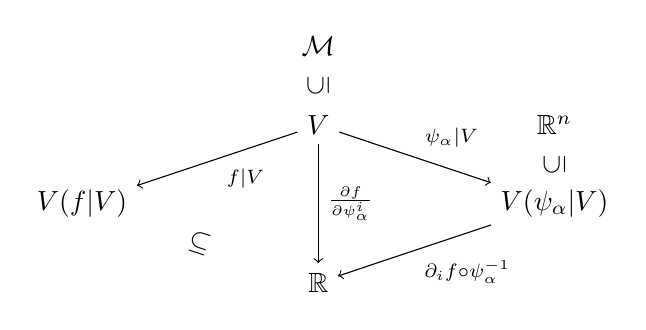
\begin{tikzpicture}[auto]
    \node (a) at ( 0, 3) {$\mathcal{M} $};
    \node (b) at ( 0, 2) {$V $};
    \node (f) at ( 0, 0) {$\mathbb{R} $};
    \node (g) at (-3, 1) {$V(f|V) $};
    \node (i) at ( 3, 2) {$\mathbb{R}^n $};
    \node (j) at ( 3, 1) {$V(\psi_\alpha |V ) $};
    \node (x) at ( 0.0, 2.5) {\rotatebox{90}{$\subseteq $}};
    \node (x) at (-1.5, 0.5) {\rotatebox{342}{$\subseteq $}};
    \node (x) at ( 3.0, 1.5) {\rotatebox{90}{$\subseteq $}};
    \draw [->] (b) to node {$\scriptstyle f|V$} (g);
    \draw [->] (b) to node {$\scriptstyle \psi_\alpha |V$} (j);
    \draw [->] (j) to node {$\scriptstyle \partial_i f\circ \psi_\alpha^{-1} $} (f);
    \draw [->] (b) to node {$\scriptstyle \frac{\partial f}{\partial \psi_\alpha^i } $} (f);
  \end{tikzpicture}
\end{center}
\begin{thm}\label{8.3.2.3}
$n$次元$C^{r}$級多様体$\left( \mathcal{M},\mathfrak{O} \right)$、$U \in \mathfrak{O}$なるその多様体$\left( \mathcal{M},\mathfrak{O} \right)$から1次元Euclid空間$E$における位相空間$\left( \mathbb{R},\mathfrak{O}_{d_{E}} \right)$への連続写像$f:U \rightarrow \mathbb{R}$、その多様体$\left( \mathcal{M},\mathfrak{O} \right)$の$C^{r}$級座標近傍系$\left\{ \left( U_{\alpha},\psi_{\alpha} \right) \right\}_{\alpha \in A}$が与えられたとする。その局所座標系$\psi_\alpha $が$\psi_\alpha =\left( \psi_\alpha^i \right)_{i\in \varLambda_n }$とおかれ、さらに、その写像$f$が、$1\leq s \leq r$としてその開集合$U$で$C^{s}$級であるとき、$\exists V\in \mathfrak{O}$に対し、$V\subseteq U\cap U_\alpha \cap U_\beta $が成り立つのであったことに注意すれば、$k\in \varLambda_n $として次式が成り立つ。
\begin{align*}
\frac{\partial f}{\partial \psi_\alpha^i } = \frac{\partial f}{\partial \psi_\beta^k } \frac{\partial \psi_\beta^k }{\partial \psi_\alpha^i } : V\rightarrow \mathbb{R}
\end{align*}
\end{thm}\par
この定理から計算方法が分かっただけではなく定義\ref{写像はCs級であることの定義}でわざわざ局所座標系を述べる必要がなかったこともわかる。
\begin{proof}
$n$次元$C^{r}$級多様体$\left( \mathcal{M},\mathfrak{O} \right)$、$U \in \mathfrak{O}$なるその多様体$\left( \mathcal{M},\mathfrak{O} \right)$から1次元Euclid空間$E$における位相空間$\left( \mathbb{R},\mathfrak{O}_{d_{E}} \right)$への連続写像$f:U \rightarrow \mathbb{R}$、その多様体$\left( \mathcal{M},\mathfrak{O} \right)$の$C^{r}$級座標近傍系$\left\{ \left( U_{\alpha},\psi_{\alpha} \right) \right\}_{\alpha \in A}$が与えられたとする。その局所座標系$\psi_\alpha $が$\psi_\alpha =\left( \psi_\alpha^i \right)_{i\in \varLambda_n }$とおかれ、さらに、その写像$f$が、$1\leq s \leq r$としてその開集合$U$で$C^{s}$級であるとき、$\exists V\in \mathfrak{O}$に対し、$V\subseteq U\cap U_\alpha \cap U_\beta $が成り立つのであったことに注意すれば、$k\in \varLambda_n $として次のようになる。
\begin{comment}
\begin{align*}
\frac{\partial f}{\partial \psi_\alpha^i } &=\partial_i \left( f|V \circ \psi_\alpha^{-1} |V \left( \psi_\alpha |V \right)\right) \circ \psi_\alpha |V \\
&=\partial_i \left( f|V \circ \left( \psi_\beta |V\right)^{-1} \circ \psi_\beta |V \circ \psi_\alpha^{-1} |V \left( \psi_\alpha |V \right)\right) \circ \psi_\alpha |V \\
&=\partial_i \left( f|V \circ \psi_\beta^{-1} |V\left( \psi_\beta |V \right) \circ \psi_\beta |V \circ \psi_\alpha^{-1} |V \left( \psi_\alpha |V \right)\right) \circ \psi_\alpha |V \\
&=\left( \partial_k \left( f|V \circ \psi_\beta^{-1} |V\left( \psi_\beta |V \right) \right) \circ \psi_\beta |V \circ \psi_\alpha^{-1} |V \left( \psi_\alpha |V \right) \right) \\
&\quad \partial_i \left( \psi_\beta^k |V \circ \psi_\alpha^{-1} |V \left( \psi_\alpha |V \right) \right) \circ \psi_\alpha |V \\
&=\left( \partial_k \left( f|V \circ \psi_\beta^{-1} |V\left( \psi_\beta |V \right) \right) \circ \psi_\beta |V \circ \left( \psi_\alpha |V \right)^{-1} \circ \psi_\alpha |V \right) \\
&\quad \left( \partial_i \left( \psi_\beta^k |V \circ \psi_\alpha^{-1} |V \left( \psi_\alpha |V \right) \right) \circ \psi_\alpha |V \right) \\
&=\left( \partial_k \left( f|V \circ \psi_\beta^{-1} |V\left( \psi_\beta |V \right) \right) \circ \psi_\beta |V \right) \\
&\quad \left( \partial_i \left( \psi_\beta^k |V \circ \psi_\alpha^{-1} |V \left( \psi_\alpha |V \right) \right) \circ \psi_\alpha |V \right) \\
&= \frac{\partial f}{\partial \psi_\beta^k } \frac{\partial \psi_\beta^k }{\partial \psi_\alpha^i }
\end{align*}
\end{comment}
\begin{align*}
  \frac{\partial f}{\partial \psi_\alpha^i } &=\partial_i \left( f\circ \psi_\alpha^{-1} \right) \circ \psi_\alpha \\
  &=\partial_i \left( f\circ \psi_\beta^{-1} \circ \psi_\beta \circ \psi_\alpha^{-1} \right) \circ \psi_\alpha \\
  &=\left( \partial_k \left( f\circ \psi_\beta^{-1} \right) \circ \psi_\beta \circ \psi_\alpha^{-1} \partial_i \left( \psi_\beta^k \circ \psi_\alpha^{-1} \right) \right) \circ \psi_\alpha \\
  &=\left( \partial_k \left( f\circ \psi_\beta^{-1} \right) \circ \psi_\beta \circ \psi_\alpha^{-1} \circ \psi_\alpha \right) \left( \partial_i \left( \psi_\beta^k \circ \psi_\alpha^{-1} \right) \circ \psi_\alpha \right) \\
  &=\left( \partial_k \left( f\circ \psi_\beta^{-1} \right) \circ \psi_\beta \right) \left( \partial_i \left( \psi_\beta^k \circ \psi_\alpha^{-1} \right) \circ \psi_\alpha \right) \\
  &= \frac{\partial f}{\partial \psi_\beta^k } \frac{\partial \psi_\beta^k }{\partial \psi_\alpha^i }
\end{align*}
\end{proof}
\begin{thm}\label{8.3.2.4}
$n$次元$C^{r}$級多様体$\left( \mathcal{M},\mathfrak{O} \right)$、その多様体$\left( \mathcal{M},\mathfrak{O} \right)$の$C^{r}$級座標近傍系$\left\{ \left( U_{\alpha},\psi_{\alpha} \right) \right\}_{\alpha \in A}$が与えられたとする。その局所座標系$\psi_\alpha $が$\psi_\alpha =\left( \psi_\alpha^i \right)_{i\in \varLambda_n }$とおかれるとき、$\exists V\in \mathfrak{O}$に対し、$V\subseteq U_\alpha \cap U_\beta $が成り立つのであったことに注意すれば、$k\in \varLambda_n $として次式が成り立つ。
\begin{align*}
  \delta_{ij} = \frac{\partial \psi_\alpha^j }{\partial \psi_\beta^k } \frac{\partial \psi_\beta^k }{\partial \psi_\alpha^i } : V\rightarrow \mathbb{R}
\end{align*}\par
さらに、次のように行列$A_{\left(U_\alpha ,\psi_\alpha \right)\rightarrow \left(U_\beta ,\psi_\beta \right)}$がおかれれば、
\begin{align*}
  A_{\left(U_\alpha ,\psi_\alpha \right)\rightarrow \left(U_\beta ,\psi_\beta \right)} = \begin{pmatrix}
    \frac{\partial \psi_\alpha^1 }{\partial \psi_\beta^1 } & \frac{\partial \psi_\alpha^2 }{\partial \psi_\beta^1 } & \cdots & \frac{\partial \psi_\alpha^n }{\partial \psi_\beta^1 } \\
    \frac{\partial \psi_\alpha^1 }{\partial \psi_\beta^2 } & \frac{\partial \psi_\alpha^2 }{\partial \psi_\beta^2 } & \cdots & \frac{\partial \psi_\alpha^n }{\partial \psi_\beta^2 } \\
    \vdots & \vdots & \ddots & \vdots \\
    \frac{\partial \psi_\alpha^1 }{\partial \psi_\beta^n } & \frac{\partial \psi_\alpha^2 }{\partial \psi_\beta^n } & \cdots & \frac{\partial \psi_\alpha^n }{\partial \psi_\beta^n } 
  \end{pmatrix} : U_\alpha \cap U_\beta \rightarrow \mathbb{R}
\end{align*}
$\det A_{\left(U_\alpha ,\psi_\alpha \right)\rightarrow \left(U_\beta ,\psi_\beta \right)} \ne 0$で$A_{\left(U_\alpha ,\psi_\alpha \right)\rightarrow \left(U_\beta ,\psi_\beta \right)}^{-1} = A_{\left(U_\beta ,\psi_\beta \right)\rightarrow \left(U_\alpha ,\psi_\alpha \right)} $が成り立つ。
\end{thm}
\begin{proof}
$n$次元$C^{r}$級多様体$\left( \mathcal{M},\mathfrak{O} \right)$、その多様体$\left( \mathcal{M},\mathfrak{O} \right)$の$C^{r}$級座標近傍系$\left\{ \left( U_{\alpha},\psi_{\alpha} \right) \right\}_{\alpha \in A}$が与えられたとする。その局所座標系$\psi_\alpha $が$\psi_\alpha =\left( \psi_\alpha^i \right)_{i\in \varLambda_n }$とおかれるとき、$\exists V\in \mathfrak{O}$に対し、$V\subseteq U_\alpha \cap U_\beta $が成り立つのであったことに注意すれば、$k\in \varLambda_n $として定理\ref{8.3.2.1}、定理\ref{8.3.2.3}より次のようになる。
\begin{align*}
  \frac{\partial \psi_\alpha^j }{\partial \psi_\alpha^i } = \frac{\partial \psi_\alpha^j }{\partial \psi_\beta^k } \frac{\partial \psi_\beta^k }{\partial \psi_\alpha^i } : V\rightarrow \mathbb{R}
\end{align*}
ここで、次のようになることから、
\begin{align*}
  \frac{\partial \psi_\alpha^j }{\partial \psi_\alpha^i } &= \partial_i \left( \psi_\alpha^j \circ \psi_\alpha^{-1} \right) \circ \psi_\alpha \\
  &= \partial_i \mathrm{pr}_j \circ \psi_\alpha = \delta_{ij} 
\end{align*}
次式が成り立つ。
\begin{align*}
  \delta_{ij} = \frac{\partial \psi_\alpha^j }{\partial \psi_\beta^k } \frac{\partial \psi_\beta^k }{\partial \psi_\alpha^i } : V\rightarrow \mathbb{R}
\end{align*}\par
さらに、次のように行列$A_{\left(U_\alpha ,\psi_\alpha \right)\rightarrow \left(U_\beta ,\psi_\beta \right)}$がおかれよう。
\begin{align*}
  A_{\left(U_\alpha ,\psi_\alpha \right)\rightarrow \left(U_\beta ,\psi_\beta \right)} = \begin{pmatrix}
    \frac{\partial \psi_\alpha^1 }{\partial \psi_\beta^1 } & \frac{\partial \psi_\alpha^2 }{\partial \psi_\beta^1 } & \cdots & \frac{\partial \psi_\alpha^n }{\partial \psi_\beta^1 } \\
    \frac{\partial \psi_\alpha^1 }{\partial \psi_\beta^2 } & \frac{\partial \psi_\alpha^2 }{\partial \psi_\beta^2 } & \cdots & \frac{\partial \psi_\alpha^n }{\partial \psi_\beta^2 } \\
    \vdots & \vdots & \ddots & \vdots \\
    \frac{\partial \psi_\alpha^1 }{\partial \psi_\beta^n } & \frac{\partial \psi_\alpha^2 }{\partial \psi_\beta^n } & \cdots & \frac{\partial \psi_\alpha^n }{\partial \psi_\beta^n } 
  \end{pmatrix} : U_\alpha \cap U_\beta \rightarrow \mathbb{R}
\end{align*}
このとき、上記の議論により次のようになる、
\begin{align*}
  \delta_{ij} = \frac{\partial \psi_\alpha^j }{\partial \psi_\beta^k } \frac{\partial \psi_\beta^k }{\partial \psi_\alpha^i } : V\rightarrow \mathbb{R},\ \ \delta_{ij} = \frac{\partial \psi_\beta^j }{\partial \psi_\alpha^k } \frac{\partial \psi_\alpha^k }{\partial \psi_\beta^i } : V\rightarrow \mathbb{R}
\end{align*}
即ち、次式が成り立つ。
\begin{align*}
  A_{\left(U_\alpha ,\psi_\alpha \right)\rightarrow \left(U_\beta ,\psi_\beta \right)} A_{\left(U_\beta ,\psi_\beta \right)\rightarrow \left(U_\alpha ,\psi_\alpha \right)} =A_{\left(U_\beta ,\psi_\beta \right)\rightarrow \left(U_\alpha ,\psi_\alpha \right)} A_{\left(U_\alpha ,\psi_\alpha \right)\rightarrow \left(U_\beta ,\psi_\beta \right)} =I_n 
\end{align*}\par
よって、$\det A_{\left(U_\alpha ,\psi_\alpha \right)\rightarrow \left(U_\beta ,\psi_\beta \right)} \ne 0$で$A_{\left(U_\alpha ,\psi_\alpha \right)\rightarrow \left(U_\beta ,\psi_\beta \right)}^{-1} = A_{\left(U_\beta ,\psi_\beta \right)\rightarrow \left(U_\alpha ,\psi_\alpha \right)} $が成り立つ。
\begin{comment}
$\det A_{\left(U_\alpha ,\psi_\alpha \right)\rightarrow \left(U_\beta ,\psi_\beta \right)} = 0$が成り立つと仮定すると、上記の議論より次のようになる。
\begin{align*}
  1 &= \det I_n =\det \begin{pmatrix}
    1 & 0 & \cdots & 0 \\
    0 & 1 & \cdots & 0 \\
    \vdots & \vdots & \ddots & \vdots \\
    0 & 0 & \cdots & 1 \\
  \end{pmatrix}\\
  &= \left| \begin{matrix}
    \frac{\partial \psi_\alpha^1 }{\partial \psi_\beta^k } \frac{\partial \psi_\beta^k }{\partial \psi_\alpha^1 } & \frac{\partial \psi_\alpha^2 }{\partial \psi_\beta^k } \frac{\partial \psi_\beta^k }{\partial \psi_\alpha^1 } & \cdots & \frac{\partial \psi_\alpha^n }{\partial \psi_\beta^k } \frac{\partial \psi_\beta^k }{\partial \psi_\alpha^1 }\\
    \frac{\partial \psi_\alpha^1 }{\partial \psi_\beta^k } \frac{\partial \psi_\beta^k }{\partial \psi_\alpha^2 } & \frac{\partial \psi_\alpha^2 }{\partial \psi_\beta^k } \frac{\partial \psi_\beta^k }{\partial \psi_\alpha^2 } & \cdots & \frac{\partial \psi_\alpha^n }{\partial \psi_\beta^k } \frac{\partial \psi_\beta^k }{\partial \psi_\alpha^2 }\\
    \vdots & \vdots & \ddots & \vdots \\
    \frac{\partial \psi_\alpha^1 }{\partial \psi_\beta^k } \frac{\partial \psi_\beta^k }{\partial \psi_\alpha^n } & \frac{\partial \psi_\alpha^2 }{\partial \psi_\beta^k } \frac{\partial \psi_\beta^k }{\partial \psi_\alpha^n } & \cdots & \frac{\partial \psi_\alpha^n }{\partial \psi_\beta^k } \frac{\partial \psi_\beta^k }{\partial \psi_\alpha^n }
  \end{matrix} \right| \\
  &= \left| \begin{matrix}
    \frac{\partial \psi_\beta^1 }{\partial \psi_\alpha^1 }& \frac{\partial \psi_\beta^2 }{\partial \psi_\alpha^1 } & \cdots & \frac{\partial \psi_\beta^n }{\partial \psi_\alpha^1 }\\
    \frac{\partial \psi_\beta^1 }{\partial \psi_\alpha^2 } & \frac{\partial \psi_\beta^2 }{\partial \psi_\alpha^2 } & \cdots & \frac{\partial \psi_\beta^n }{\partial \psi_\alpha^2 }\\
    \vdots & \vdots & \ddots & \vdots \\
    \frac{\partial \psi_\beta^1 }{\partial \psi_\alpha^n } & \frac{\partial \psi_\beta^2 }{\partial \psi_\alpha^n }\circ \psi_\alpha^{-1} & \cdots & \frac{\partial \psi_\beta^n }{\partial \psi_\alpha^n }
  \end{matrix} \right| \left| \begin{matrix}
    \frac{\partial \psi_\alpha^1 }{\partial \psi_\beta^1 } & \frac{\partial \psi_\alpha^2 }{\partial \psi_\beta^1 } & \cdots & \frac{\partial \psi_\alpha^n }{\partial \psi_\beta^1 }\\
    \frac{\partial \psi_\alpha^1 }{\partial \psi_\beta^2 } & \frac{\partial \psi_\alpha^2 }{\partial \psi_\beta^2 } & \cdots & \frac{\partial \psi_\alpha^n }{\partial \psi_\beta^2 } \\
    \vdots & \vdots & \ddots & \vdots \\
    \frac{\partial \psi_\alpha^1 }{\partial \psi_\beta^n } & \frac{\partial \psi_\alpha^2 }{\partial \psi_\beta^n } & \cdots & \frac{\partial \psi_\alpha^n }{\partial \psi_\beta^n }
  \end{matrix} \right| \\
\end{align*}
ここで、仮定より次式が成り立つので、
\begin{align*}
  \det A_{\left(U_\alpha ,\psi_\alpha \right)\rightarrow \left(U_\beta ,\psi_\beta \right)} \circ \psi_\alpha^{-1} = \left| \begin{matrix}
    \frac{\partial \psi_\alpha^1 }{\partial \psi_\beta^1 } \circ \psi_\alpha^{-1} & \frac{\partial \psi_\alpha^2 }{\partial \psi_\beta^1 } \circ \psi_\alpha^{-1} & \cdots & \frac{\partial \psi_\alpha^n }{\partial \psi_\beta^1 } \circ \psi_\alpha^{-1} \\
    \frac{\partial \psi_\alpha^1 }{\partial \psi_\beta^2 } \circ \psi_\alpha^{-1} & \frac{\partial \psi_\alpha^2 }{\partial \psi_\beta^2 } \circ \psi_\alpha^{-1} & \cdots & \frac{\partial \psi_\alpha^n }{\partial \psi_\beta^2 } \circ \psi_\alpha^{-1} \\
    \vdots & \vdots & \ddots & \vdots \\
    \frac{\partial \psi_\alpha^1 }{\partial \psi_\beta^n } \circ \psi_\alpha^{-1} & \frac{\partial \psi_\alpha^2 }{\partial \psi_\beta^n } \circ \psi_\alpha^{-1} & \cdots & \frac{\partial \psi_\alpha^n }{\partial \psi_\beta^n } \circ \psi_\alpha^{-1}
  \end{matrix} \right| =0
\end{align*}
$1 = 0$が得られるが、これは矛盾している。よって、$\det A_{\left(U_\alpha ,\psi_\alpha \right)\rightarrow \left(U_\beta ,\psi_\beta \right)} \ne 0$が成り立つ。
\end{comment}
\end{proof}
\subsubsection{関数行列式}
\begin{dfn}
$n$次元$C^{r}$級多様体$\left( \mathcal{M},\mathfrak{O} \right)$、$U \in \mathfrak{O}$なるその多様体$\left( \mathcal{M},\mathfrak{O} \right)$から1次元Euclid空間$E$における位相空間$\left( \mathbb{R},\mathfrak{O}_{d_{E}} \right)$への$1\leq s \leq r$としてその開集合$U$で$C^{s}$級な写像の族$\left\{ f_i :U \rightarrow \mathbb{R} \right\}_{i\in \varLambda_n } $、その多様体$\left( \mathcal{M},\mathfrak{O} \right)$の$C^{r}$級座標近傍系$\left\{ \left( U_{\alpha},\psi_{\alpha} \right) \right\}_{\alpha \in A}$が与えられたとする。写像$\left( f_i \right)_{i\in \varLambda_n } :U \rightarrow \mathbb{R}^n $が$f:U \rightarrow \mathbb{R}^n $\footnote{もちろん、その写像$f$がその開集合$U$で微分可能でJacobi行列をもつのであれば、その族$\left\{ f_i \right\}_{i\in \varLambda_n } $のどの元はその開集合$U$で$C^1$級です。}、その局所座標系$\psi_\alpha $が$\psi_\alpha =\left( \psi_\alpha^i \right)_{i\in \varLambda_n }$とおかれ、$U\cap U_\alpha \ne \emptyset $のとき\footnote{定理\ref{8.3.1.3}より$\exists \alpha \in A$に対し、$U\cap U_\alpha \ne \emptyset $が成り立ちます。}、次のように写像$\frac{Df}{D\psi_\alpha }$が定義される。その写像$\frac{Df}{D\psi_\alpha }$をその写像$f$のその座標近傍$\left(U_\alpha ,\psi_\alpha \right)$におけるその開集合$U$での関数行列式という。
\begin{align*}
\frac{Df}{D\psi_\alpha } =\left| \begin{matrix}
  \frac{\partial f^1 }{\partial \psi_\alpha^1 } & \frac{\partial f^1 }{\partial \psi_\alpha^2 } & \cdots & \frac{\partial f^1 }{\partial \psi_\alpha^n } \\
  \frac{\partial f^2 }{\partial \psi_\alpha^1 } & \frac{\partial f^2 }{\partial \psi_\alpha^2 } & \cdots & \frac{\partial f^2 }{\partial \psi_\alpha^n } \\
  \vdots & \vdots & \ddots & \vdots \\
  \frac{\partial f^n }{\partial \psi_\alpha^1 } & \frac{\partial f^n }{\partial \psi_\alpha^2 } & \cdots & \frac{\partial f^n }{\partial \psi_\alpha^n }
\end{matrix} \right| :U\cap U_\alpha \rightarrow \mathbb{R}
\end{align*}
\end{dfn}
\begin{thm}\label{8.3.2.5}
$n$次元$C^{r}$級多様体$\left( \mathcal{M},\mathfrak{O} \right)$、$U \in \mathfrak{O}$なるその多様体$\left( \mathcal{M},\mathfrak{O} \right)$から1次元Euclid空間$E$における位相空間$\left( \mathbb{R},\mathfrak{O}_{d_{E}} \right)$への$1\leq s \leq r$としてその開集合$U$で$C^{s}$級な写像の族$\left\{ f_i :U \rightarrow \mathbb{R} \right\}_{i\in \varLambda_n } $、その多様体$\left( \mathcal{M},\mathfrak{O} \right)$の$C^{r}$級座標近傍系$\left\{ \left( U_{\alpha},\psi_{\alpha} \right) \right\}_{\alpha \in A}$が与えられたとする。写像$\left( f_i \right)_{i\in \varLambda_n } :U \rightarrow \mathbb{R}^n $が$f:U \rightarrow \mathbb{R}^n $、その局所座標系$\psi_\alpha $が$\psi_\alpha =\left( \psi_\alpha^i \right)_{i\in \varLambda_n }$とおかれ、$U\cap U_\alpha \cap U_\beta \ne \emptyset $のとき、次式が成り立つ。
\begin{align*}
\frac{Df}{D\psi_\beta } = \det A_{\left(U_\alpha ,\psi_\alpha \right)\rightarrow \left(U_\beta ,\psi_\beta \right)} \frac{Df}{D\psi_\alpha } : U\cap U_\alpha \cap U_\beta \rightarrow \mathbb{R}
\end{align*}
特に、$\frac{Df}{D\psi_\alpha } |U\cap U_\alpha \cap U_\beta \ne 0$が成り立つのであれば、$\frac{Df}{D\psi_\beta } |U\cap U_\alpha \cap U_\beta \ne 0$も成り立つことになる。
\end{thm}
\begin{proof}
$n$次元$C^{r}$級多様体$\left( \mathcal{M},\mathfrak{O} \right)$、$U \in \mathfrak{O}$なるその多様体$\left( \mathcal{M},\mathfrak{O} \right)$から1次元Euclid空間$E$における位相空間$\left( \mathbb{R},\mathfrak{O}_{d_{E}} \right)$への$1\leq s \leq r$としてその開集合$U$で$C^{s}$級な写像の族$\left\{ f_i :U \rightarrow \mathbb{R} \right\}_{i\in \varLambda_n } $、その多様体$\left( \mathcal{M},\mathfrak{O} \right)$の$C^{r}$級座標近傍系$\left\{ \left( U_{\alpha},\psi_{\alpha} \right) \right\}_{\alpha \in A}$が与えられたとする。写像$\left( f_i \right)_{i\in \varLambda_n } :U \rightarrow \mathbb{R}^n $が$f:U \rightarrow \mathbb{R}^n $、その局所座標系$\psi_\alpha $が$\psi_\alpha =\left( \psi_\alpha^i \right)_{i\in \varLambda_n }$とおかれ、$U\cap U_\alpha \cap U_\beta \ne \emptyset $のとき、$\forall i,j\in \varLambda_n $に対し、定理\ref{8.3.2.3}より次式が成り立つ。
\begin{align*}
\frac{\partial f^i }{\partial \psi_\beta^j } = \frac{\partial f^i }{\partial \psi_\alpha^k } \frac{\partial \psi_\alpha^k }{\partial \psi_\beta^j } 
\end{align*}
したがって、次式が成り立つので、
\begin{align*}
\left| \begin{matrix}
  \frac{\partial f^1 }{\partial \psi_\beta^1 } & \frac{\partial f^1 }{\partial \psi_\beta^2 } & \cdots & \frac{\partial f^1 }{\partial \psi_\beta^n } \\
  \frac{\partial f^2 }{\partial \psi_\beta^1 } & \frac{\partial f^2 }{\partial \psi_\beta^2 } & \cdots & \frac{\partial f^2 }{\partial \psi_\beta^n } \\
  \vdots & \vdots & \ddots & \vdots \\
  \frac{\partial f^n }{\partial \psi_\beta^1 } & \frac{\partial f^n }{\partial \psi_\beta^2 } & \cdots & \frac{\partial f^n }{\partial \psi_\beta^n }
\end{matrix} \right| &= \left| \begin{matrix}
  \frac{\partial f^1 }{\partial \psi_\alpha^k } \frac{\partial \psi_\alpha^k }{\partial \psi_\beta^1 } & \frac{\partial f^1 }{\partial \psi_\alpha^k } \frac{\partial \psi_\alpha^k }{\partial \psi_\beta^2 }  & \cdots & \frac{\partial f^1 }{\partial \psi_\alpha^k } \frac{\partial \psi_\alpha^k }{\partial \psi_\beta^n }  \\
  \frac{\partial f^2 }{\partial \psi_\alpha^k } \frac{\partial \psi_\alpha^k }{\partial \psi_\beta^1 }  & \frac{\partial f^2 }{\partial \psi_\alpha^k } \frac{\partial \psi_\alpha^k }{\partial \psi_\beta^2 }  & \cdots & \frac{\partial f^2 }{\partial \psi_\alpha^k } \frac{\partial \psi_\alpha^k }{\partial \psi_\beta^n }  \\
  \vdots & \vdots & \ddots & \vdots \\
  \frac{\partial f^n }{\partial \psi_\alpha^k } \frac{\partial \psi_\alpha^k }{\partial \psi_\beta^1 }  & \frac{\partial f^n }{\partial \psi_\alpha^k } \frac{\partial \psi_\alpha^k }{\partial \psi_\beta^2 }  & \cdots & \frac{\partial f^n }{\partial \psi_\alpha^k } \frac{\partial \psi_\alpha^k }{\partial \psi_\beta^n } 
\end{matrix} \right| \\
&= \left| \begin{matrix}
  \frac{\partial f^1 }{\partial \psi_\alpha^1 } & \frac{\partial f^1 }{\partial \psi_\alpha^2 }  & \cdots & \frac{\partial f^1 }{\partial \psi_\alpha^n } \\
  \frac{\partial f^2 }{\partial \psi_\alpha^1 } & \frac{\partial f^2 }{\partial \psi_\alpha^2 } & \cdots & \frac{\partial f^2 }{\partial \psi_\alpha^n } \\
  \vdots & \vdots & \ddots & \vdots \\
  \frac{\partial f^n }{\partial \psi_\alpha^1 }  & \frac{\partial f^n }{\partial \psi_\alpha^2 }  & \cdots & \frac{\partial f^n }{\partial \psi_\alpha^n } 
\end{matrix} \right| \left| \begin{matrix}
  \frac{\partial \psi_\alpha^1 }{\partial \psi_\beta^1 } & \frac{\partial \psi_\alpha^1 }{\partial \psi_\beta^2 }  & \cdots & \frac{\partial \psi_\alpha^1 }{\partial \psi_\beta^n }  \\
  \frac{\partial \psi_\alpha^2 }{\partial \psi_\beta^1 }  & \frac{\partial \psi_\alpha^2 }{\partial \psi_\beta^2 }  & \cdots & \frac{\partial \psi_\alpha^2 }{\partial \psi_\beta^n }  \\
  \vdots & \vdots & \ddots & \vdots \\
  \frac{\partial \psi_\alpha^n }{\partial \psi_\beta^1 }  & \frac{\partial \psi_\alpha^n }{\partial \psi_\beta^2 }  & \cdots & \frac{\partial \psi_\alpha^n }{\partial \psi_\beta^n } \end{matrix} \right| \\
&= \left| \begin{matrix}
  \frac{\partial \psi_\alpha^1 }{\partial \psi_\beta^1 } & \frac{\partial \psi_\alpha^2 }{\partial \psi_\beta^1 } & \cdots & \frac{\partial \psi_\alpha^n }{\partial \psi_\beta^1 } \\
  \frac{\partial \psi_\alpha^1 }{\partial \psi_\beta^2 } & \frac{\partial \psi_\alpha^2 }{\partial \psi_\beta^2 } & \cdots & \frac{\partial \psi_\alpha^n }{\partial \psi_\beta^2 } \\
  \vdots & \vdots & \ddots & \vdots \\
  \frac{\partial \psi_\alpha^1 }{\partial \psi_\beta^n } & \frac{\partial \psi_\alpha^2 }{\partial \psi_\beta^n } & \cdots & \frac{\partial \psi_\alpha^n }{\partial \psi_\beta^n } \\
\end{matrix} \right| \left| \begin{matrix}
  \frac{\partial f^1 }{\partial \psi_\alpha^1 } & \frac{\partial f^1 }{\partial \psi_\alpha^2 }  & \cdots & \frac{\partial f^1 }{\partial \psi_\alpha^n } \\
  \frac{\partial f^2 }{\partial \psi_\alpha^1 } & \frac{\partial f^2 }{\partial \psi_\alpha^2 } & \cdots & \frac{\partial f^2 }{\partial \psi_\alpha^n } \\
  \vdots & \vdots & \ddots & \vdots \\
  \frac{\partial f^n }{\partial \psi_\alpha^1 }  & \frac{\partial f^n }{\partial \psi_\alpha^2 }  & \cdots & \frac{\partial f^n }{\partial \psi_\alpha^n } 
\end{matrix} \right|
\end{align*}
次式が成り立つ。
\begin{align*}
\frac{Df}{D\psi_\beta } = \det A_{\left(U_\alpha ,\psi_\alpha \right)\rightarrow \left(U_\beta ,\psi_\beta \right)} \frac{Df}{D\psi_\alpha } 
\end{align*}\par
特に、$\frac{Df}{D\psi_\alpha } |U\cap U_\alpha \cap U_\beta \ne 0$が成り立つのであれば、定理\ref{8.3.2.4}より$\frac{Df}{D\psi_\beta } |U\cap U_\alpha \cap U_\beta \ne 0$も成り立つことになる。
\end{proof}
\begin{thm}\label{8.3.2.6}
$n$次元$C^{r}$級多様体$\left( \mathcal{M},\mathfrak{O} \right)$、その多様体$\left( \mathcal{M},\mathfrak{O} \right)$の$C^{r}$級座標近傍系$\left\{ \left( U_{\alpha},\psi_{\alpha} \right) \right\}_{\alpha \in A}$が与えられたとする。その局所座標系$\psi_\alpha $が$\psi_\alpha =\left( \psi_\alpha^i \right)_{i\in \varLambda_n }$とおかれたとき、$\frac{D\psi_\alpha }{D\psi_\alpha } = 1 $が成り立つ。
\end{thm}
\begin{proof}
$n$次元$C^{r}$級多様体$\left( \mathcal{M},\mathfrak{O} \right)$、その多様体$\left( \mathcal{M},\mathfrak{O} \right)$の$C^{r}$級座標近傍系$\left\{ \left( U_{\alpha},\psi_{\alpha} \right) \right\}_{\alpha \in A}$が与えられたとする。その局所座標系$\psi_\alpha $が$\psi_\alpha =\left( \psi_\alpha^i \right)_{i\in \varLambda_n }$とおかれたとき、定理\ref{8.3.2.1}に注意すれば、$\forall i,j\in \varLambda_n $に対し、$\frac{\partial \psi_\alpha^i }{\partial \psi_\alpha^j } $が定義できて次のようになるので、
\begin{align*}
\frac{\partial \psi_\alpha^i }{\partial \psi_\alpha^j } &= \partial_j \left( \psi_\alpha^i \circ \psi_\alpha^{-1} \right) \circ \psi_\alpha \\
&= \partial_j \mathrm{pr}_i \circ \psi_\alpha = \delta_{ij} 
\end{align*}
$\frac{D\psi_\alpha }{D\psi_\alpha } \circ \psi_\alpha^{-1} = 1 $が成り立つ。
\end{proof}
\begin{dfn}
$n$次元$C^{r}$級多様体$\left( \mathcal{M},\mathfrak{O} \right)$、$U \in \mathfrak{O}$なるその多様体$\left( \mathcal{M},\mathfrak{O} \right)$から1次元Euclid空間$E$における位相空間$\left( \mathbb{R},\mathfrak{O}_{d_{E}} \right)$への$1\leq s \leq r$としてその開集合$U$で$C^{s}$級な写像の族$\left\{ f_i :U \rightarrow \mathbb{R} \right\}_{i\in \varLambda_n } $、その多様体$\left( \mathcal{M},\mathfrak{O} \right)$の$C^{r}$級座標近傍系$\left\{ \left( U_{\alpha},\psi_{\alpha} \right) \right\}_{\alpha \in A}$が与えられたとする。写像$\left( f_i \right)_{i\in \varLambda_n } :U \rightarrow \mathbb{R}^n $が$f:U \rightarrow \mathbb{R}^n $、その局所座標系$\psi_\alpha $が$\psi_\alpha =\left( \psi_\alpha^i \right)_{i\in \varLambda_n }$とおかれ、$U\cap U_\alpha \ne \emptyset $のとき、その写像$f$のその座標近傍$\left(U_\alpha ,\psi_\alpha \right)$におけるその開集合$U$での関数行列式$\frac{Df}{D\psi_\alpha }$が$p\in U\cap U_\alpha $なる元$p$で$\frac{Df}{D\psi_\alpha } (p) \ne 0$を満たすとき、その写像$f$をその元$p$のまわりの$C^s $級局所座標系という。
\end{dfn}
\begin{thm}\label{8.3.2.7}
$n$次元$C^{r}$級多様体$\left( \mathcal{M},\mathfrak{O} \right)$、$U \in \mathfrak{O}$なるその多様体$\left( \mathcal{M},\mathfrak{O} \right)$から1次元Euclid空間$E$における位相空間$\left( \mathbb{R},\mathfrak{O}_{d_{E}} \right)$への$1\leq s \leq r$としてその開集合$U$で$C^{s}$級な写像の族$\left\{ f_i :U \rightarrow \mathbb{R} \right\}_{i\in \varLambda_n } $、その多様体$\left( \mathcal{M},\mathfrak{O} \right)$の$C^{r}$級座標近傍系$\left\{ \left( U_{\alpha},\psi_{\alpha} \right) \right\}_{\alpha \in A}$が与えられたとする。写像$\left( f_i \right)_{i\in \varLambda_n } :U \rightarrow \mathbb{R}^n $が$f:U \rightarrow \mathbb{R}^n $、その局所座標系$\psi_\alpha $が$\psi_\alpha =\left( \psi_\alpha^i \right)_{i\in \varLambda_n }$とおかれ、$U\cap U_\alpha \ne \emptyset $のとき、その写像$f$のその座標近傍$\left(U_\alpha ,\psi_\alpha \right)$におけるその開集合$U$での関数行列式$\frac{Df}{D\psi_\alpha }$が$p\in U\cap U_\alpha $なる元$p$で$\frac{Df}{D\psi_\alpha } (p) \ne 0$を満たすとき、その部分位相空間$\left( U\cap U_\alpha ,\mathfrak{O}_{U\cap U_\alpha } \right)$におけるその元$p$のある近傍$V$が存在して、$\frac{Df}{D\psi_\alpha } |V \ne 0$が成り立つ。
\end{thm}\par
このことから、その写像$f$がその元$p$のまわりの$C^s $級局所座標系であれば、その元$p$の近傍$V$をうまくとったときのその近傍$V$の各点のまわりの$C^s $級局所座標系となる。
\begin{proof}
$n$次元$C^{r}$級多様体$\left( \mathcal{M},\mathfrak{O} \right)$、$U \in \mathfrak{O}$なるその多様体$\left( \mathcal{M},\mathfrak{O} \right)$から1次元Euclid空間$E$における位相空間$\left( \mathbb{R},\mathfrak{O}_{d_{E}} \right)$への$1\leq s \leq r$としてその開集合$U$で$C^{s}$級な写像の族$\left\{ f_i :U \rightarrow \mathbb{R} \right\}_{i\in \varLambda_n } $、その多様体$\left( \mathcal{M},\mathfrak{O} \right)$の$C^{r}$級座標近傍系$\left\{ \left( U_{\alpha},\psi_{\alpha} \right) \right\}_{\alpha \in A}$が与えられたとする。写像$\left( f_i \right)_{i\in \varLambda_n } :U \rightarrow \mathbb{R}^n $が$f:U \rightarrow \mathbb{R}^n $、その局所座標系$\psi_\alpha $が$\psi_\alpha =\left( \psi_\alpha^i \right)_{i\in \varLambda_n }$とおかれ、$U\cap U_\alpha \ne \emptyset $のとき、その写像$f$のその座標近傍$\left(U_\alpha ,\psi_\alpha \right)$におけるその開集合$U$での関数行列式$\frac{Df}{D\psi_\alpha }$が$p\in U\cap U_\alpha $なる元$p$で$\frac{Df}{D\psi_\alpha } (p) \ne 0$を満たすとき、次式が成り立つことから、
\begin{align*}
\frac{Df}{D\psi_\alpha } = \sum_{\sigma \in \mathfrak{S}_n } \mathrm{sgn} \sigma \prod_{i\in \varLambda_n } \frac{\partial f^i }{\partial \psi_\alpha^{\sigma (i)} } : U\cap U_\alpha \rightarrow \mathbb{R}
\end{align*}その関数行列式$\frac{Df}{D\psi_\alpha }$はその開集合$U\cap U_\alpha $で連続である。したがって、定理\ref{8.1.3.1}よりその元$\frac{Df}{D\psi_\alpha }(p)$の1次元Euclid空間における位相空間$\left( \mathbb{R} ,\mathfrak{O}_{d_E } \right)$におけるどの近傍$W$をとってもその値域$V\left({\frac{Df}{D\psi_\alpha } }^{-1} | W\right) $はその元$p$の近傍となる。ここで、1次元Euclid空間は距離空間なので、定理\ref{8.2.1.6}より$\exists \delta \in \mathbb{R}^+ $に対し、$B\left(\frac{Df}{D\psi_\alpha }(p) ,\delta \right) \subseteq W$が成り立つので、その値域$V\left({\frac{Df}{D\psi_\alpha } }^{-1} | B\left(\frac{Df}{D\psi_\alpha }(p) ,\delta \right) \right) $もその元$p$の近傍となる。ここで、次のように正の実数$\varepsilon$が定義されれば、
\begin{align*}
\varepsilon = \min \left\{ \frac{1}{2} \left| \frac{Df}{D\psi_\alpha }(p) \right| ,\delta \right\}
\end{align*}
$B\left(\frac{Df}{D\psi_\alpha }(p) ,\varepsilon \right) \subseteq B\left(\frac{Df}{D\psi_\alpha }(p) ,\delta \right) $が成り立つので、その値域$V\left({\frac{Df}{D\psi_\alpha } }^{-1} | B\left(\frac{Df}{D\psi_\alpha }(p) ,\varepsilon \right) \right) $もその元$p$の近傍となる。ここで、この近傍を$V$とおくと、$\forall q\in V$に対し、$\frac{Df}{D\psi_\alpha }(q) \in B\left(\frac{Df}{D\psi_\alpha }(p) ,\varepsilon \right) $が成り立つので、次のようになる。
\begin{align*}
q\in V &\Leftrightarrow \frac{Df}{D\psi_\alpha }(q) \in B\left(\frac{Df}{D\psi_\alpha }(p) ,\varepsilon \right) \\
&\Leftrightarrow \left| \frac{Df}{D\psi_\alpha }(p) - \frac{Df}{D\psi_\alpha }(q) \right| < \varepsilon\leq \frac{1}{2} \left| \frac{Df}{D\psi_\alpha }(p) \right| \\
&\Rightarrow -\frac{1}{2} \left| \frac{Df}{D\psi_\alpha }(p) \right| < \left| \frac{Df}{D\psi_\alpha }(q) \right| - \left| \frac{Df}{D\psi_\alpha }(p) \right| < \frac{1}{2} \left| \frac{Df}{D\psi_\alpha }(p) \right| \\
&\Rightarrow 0 < \frac{1}{2} \left| \frac{Df}{D\psi_\alpha }(p) \right| < \left| \frac{Df}{D\psi_\alpha }(q) \right|
\end{align*}
よって、その部分位相空間$\left( U\cap U_\alpha ,\mathfrak{O}_{U\cap U_\alpha } \right)$におけるその元$p$のある近傍$V$が存在して、$\frac{Df}{D\psi_\alpha } |V \ne 0$が成り立つ。
\end{proof}
\begin{thm}\label{8.3.2.8}
$n$次元$C^{r}$級多様体$\left( \mathcal{M},\mathfrak{O} \right)$、$U \in \mathfrak{O}$なるその多様体$\left( \mathcal{M},\mathfrak{O} \right)$から1次元Euclid空間$E$における位相空間$\left( \mathbb{R},\mathfrak{O}_{d_{E}} \right)$への$1\leq s \leq r$としてその開集合$U$で$C^{s}$級な写像の族$\left\{ f_i :U \rightarrow \mathbb{R} \right\}_{i\in \varLambda_n } $、その多様体$\left( \mathcal{M},\mathfrak{O} \right)$の$C^{r}$級座標近傍系$\left\{ \left( U_{\alpha},\psi_{\alpha} \right) \right\}_{\alpha \in A}$が与えられたとする。写像$\left( f_i \right)_{i\in \varLambda_n } :U \rightarrow \mathbb{R}^n $が$f:U \rightarrow \mathbb{R}^n $、その局所座標系$\psi_\alpha $が$\psi_\alpha =\left( \psi_\alpha^i \right)_{i\in \varLambda_n }$とおかれ、$U\cap U_\alpha \ne \emptyset $でその写像$f$のその座標近傍$\left(U_\alpha ,\psi_\alpha \right)$におけるその開集合$U$での関数行列式$\frac{Df}{D\psi_\alpha }$が$p\in U\cap U_\alpha $なる元$p$で$\frac{Df}{D\psi_\alpha } (p) \ne 0$を満たすとき、即ち、その元$p$がその写像$f$の$C^s$級局所座標系であるとき、その位相空間$\left( U\cap U_\alpha ,\mathfrak{O}_{U\cap U_\alpha } \right)$におけるその元$p$のある近傍$U'$が存在して、その組$\left(U',f\right)$がその多様体$\left(\mathcal{M},\mathfrak{O}\right)$の座標近傍となる。
\end{thm}
\begin{proof}
$n$次元$C^{r}$級多様体$\left( \mathcal{M},\mathfrak{O} \right)$、$U \in \mathfrak{O}$なるその多様体$\left( \mathcal{M},\mathfrak{O} \right)$から1次元Euclid空間$E$における位相空間$\left( \mathbb{R},\mathfrak{O}_{d_{E}} \right)$への$1\leq s \leq r$としてその開集合$U$で$C^{s}$級な写像の族$\left\{ f_i :U \rightarrow \mathbb{R} \right\}_{i\in \varLambda_n } $、その多様体$\left( \mathcal{M},\mathfrak{O} \right)$の$C^{r}$級座標近傍系$\left\{ \left( U_{\alpha},\psi_{\alpha} \right) \right\}_{\alpha \in A}$が与えられたとする。写像$\left( f_i \right)_{i\in \varLambda_n } :U \rightarrow \mathbb{R}^n $が$f:U \rightarrow \mathbb{R}^n $、その局所座標系$\psi_\alpha $が$\psi_\alpha =\left( \psi_\alpha^i \right)_{i\in \varLambda_n }$とおかれ、$U\cap U_\alpha \ne \emptyset $でその写像$f$のその座標近傍$\left(U_\alpha ,\psi_\alpha \right)$におけるその開集合$U$での関数行列式$\frac{Df}{D\psi_\alpha }$が$p\in U\cap U_\alpha $なる元$p$で$\frac{Df}{D\psi_\alpha } (p) \ne 0$を満たすとき、即ち、その元$p$がその写像$f$の$C^s$級局所座標系であるとき、$\forall i,j\in \varLambda_n $に対し、次式が成り立つので、
\begin{align*}
\frac{\partial f^i }{\partial \psi_\alpha^j } = \partial_j \left( f^i \circ \psi_\alpha^{-1} \right) \circ \psi_\alpha
\end{align*}
次式が成り立つ。
\begin{align*}
\frac{Df}{D\psi_\alpha } = \det J_{f\circ \psi_\alpha^{-1} } \circ \psi_\alpha :U\cap U_\alpha \rightarrow \mathbb{R}
\end{align*}
関数行列式$\frac{Df}{D\psi_\alpha }$が$p\in U\cap U_\alpha $なる元$p$で$\frac{Df}{D\psi_\alpha } (p) \ne 0$を満たすので、$\det J_{f\circ \psi_\alpha^{-1} } \ne 0$が成り立つ、即ち、$J_{f\circ \psi_\alpha^{-1} } :U\cap U_\alpha \rightarrow M_{nn}\left(\mathbb{R}\right)$の逆行列が存在することになる。また、それらの写像たち$f_i $いずれも$C^s$級である、即ち、それらの関数たち$f_i \circ \psi_\alpha^{-1} $いずれも$C^s $級であるので、これが成り立つならそのときに限り、その関数$f\circ \psi_\alpha^{-1}$も$C^s$級である。そこで、逆関数定理より$n$次元Euclid空間$E^n $における位相空間$\left(\mathbb{R}^n ,\mathfrak{O}_{d_{E^n}}\right)$でのある開近傍たち$V$、$W$が存在して、$f\circ \psi_\alpha^{-1} |V : V\rightarrow W$の逆関数が存在するようにすることができる。さらに、その逆関数$\left(f\circ \psi_\alpha^{-1} \right)^{-1} $も$C^s$級である。特に、その関数$f\circ \psi_\alpha^{-1} $は連続でその逆関数$\left(f\circ \psi_\alpha^{-1} \right)^{-1} $も連続であるので、その関数$f\circ \psi_\alpha^{-1} $は$n$次元Euclid空間$E^n $における部分位相空間間の同相写像となっている。そこで、$U' = V\left( \psi_\alpha^{-1} |V \right)$とすれば、その写像$\psi_\alpha $が連続なのでこれは開集合で次のようになることから、
\begin{align*}
f|U' &= f \circ \psi_\alpha^{-1} \circ \psi_\alpha |V\left( \psi_\alpha^{-1} |V \right) \\
&= f \circ \psi_\alpha^{-1} |V \circ \psi_\alpha |V\left( \psi_\alpha^{-1} |V \right) 
\end{align*}
その写像$f|U'$はその部分位相空間$\left(V\left( \psi_\alpha^{-1} |V \right) , \mathfrak{O}_{V\left( \psi_\alpha^{-1} |V \right) } \right)$からその部分位相空間$\left(V,\left(\mathfrak{O}_{d_{E^n}}\right)_{V}\right)$への同相写像$\psi_\alpha |V\left( \psi_\alpha^{-1} |V \right) $とその部分位相空間$\left(V,\left(\mathfrak{O}_{d_{E^n}}\right)_{V}\right)$からその部分位相空間$\left(W,\left(\mathfrak{O}_{d_{E^n}}\right)_{W}\right)$への同相写像の合成写像となっているので、その写像$f|U'$も同相写像である。よって、その位相空間$\left( U\cap U_\alpha ,\mathfrak{O}_{U\cap U_\alpha } \right)$におけるその元$p$のある近傍$U'$が存在して、その組$\left(U',f\right)$がその多様体$\left(\mathcal{M},\mathfrak{O}\right)$の座標近傍となる。
\end{proof}
\begin{thebibliography}{50}
\bibitem{1}
  松島与三, 多様体入門, 裳華房, 1965. 第36刷 p31-35 ISBN978-4-7853-1305-0
\bibitem{2}
  新井朝雄, 相対性理論の数理, 日本評論会, 2021. 第1版第1刷 p164-166 ISBN978-4-535-78928-9
\end{thebibliography}
\end{document}
